% $Header: /projects/VU-SAGA/Papers/saga_engine_2006/saga_engine.tex,v 1.15 2006/08/13 18:01:00 hkaiser Exp $

\documentclass{acm_proc_article-sp}

\usepackage{ifpdf}
\usepackage{srcltx}
\usepackage{fancyvrb}

\ifpdf
  \usepackage{graphicx}
  \usepackage[pdftex]{hyperref}
  \DeclareGraphicsExtensions{.pdf, .png, .jpg, .JPG}
\else
  \usepackage{graphicx}
  \usepackage[hypertex]{hyperref}
  \DeclareGraphicsExtensions{.ps, .eps}
\fi
  
\newcommand{\I}{\textit}
\newcommand{\B}{\textbf}
\newcommand{\T}{\texttt}

\newcommand{\IB}[1]{\textbf{\textit{#1}}}

\newcommand{\F}[1]{\B{FIXME: #1}}

\newcommand{\up}{\vspace*{-1em}}
\newcommand{\down}{\vspace*{1em}}

\newenvironment{shortlist}{
  \begin{itemize}
  \setlength{\itemsep}{-0.2em}
}{
  \end{itemize}
}

\setlength{\floatsep}{1em}
\setlength{\textfloatsep}{1em}
\setlength{\intextsep}{1.3em}

\DefineShortVerb{\|}
\DefineVerbatimEnvironment{mycode}{Verbatim}
{
  label=Code Example,
  fontsize=\small,
  frame=single,
% framerule=1pt,
  framesep=1em,
% numbers=left,
  gobble=2
}


\pagestyle{plain}

% -------------------------------------------------------------------

\begin{document}

\title{The SAGA C++ Reference Implementation}
\subtitle{Lessons Learnt from Juggling with Seemingly Contradictory Goals}

\numberofauthors{4}
\author{
  \alignauthor Hartmut Kaiser\\
  \affaddr{Center for Computation \& Technology}\\
  \affaddr{Louisiana State University}\\
  \affaddr{Baton Rouge, Louisiana, USA}\\
  \email{\normalsize\T{hkaiser@cct.lsu.edu}}
  \alignauthor Andre Merzky\\
  \affaddr{Vrije Universiteit, Amsterdam}\\
  \affaddr{Amsterdam, The Netherlands}\\
  \email{\normalsize\T{andre@merzky.net}}
  \alignauthor Stephan Hirmer\\
  \affaddr{Center for Computation \& Technology}\\
  \affaddr{Louisiana State University}\\
  \affaddr{Baton Rouge, Louisiana, USA}\\
  \email{\normalsize\T{shirmer@cct.lsu.edu}}
}
\additionalauthors{
  \B{Gabriele Allen}\\
  \hspace*{2em}Center for Computation \& Technology\\
  \hspace*{2em}Louisiana State University\\
  \hspace*{2em}Baton Rouge, Louisiana, USA\\
  \hspace*{2em}email: \texttt{gallen@cct.lsu.edu}
  }

\date{}

\maketitle

\begin{abstract} 

  The Simple API for Grid Applications (SAGA)~\cite{saga_spec} is an ongoing API
  standardization effort within the Open Grid Forum (OGF)~\cite{ogf_website}.  
  The OGF strives to standardize grid middleware, meaning grid service
  interfaces, grid enabled protocols, and grid architecture in
  general.  As of now, most grid standard specifications are in flux,
  and furthermore there exist multiple, incompatible grid middleware
  systems which are deployed in large research or production
  environments.  SAGA is supposed to provide a simple API to
  programmers of scientific applications, allowing them to use higher
  level grid computing paradigms, and thus shielding the programmer
  and the application from the diversity and dynamicity of Grid
  environments.
  
  The SAGA specification itself is expected to extend in scope over
  the next couple of years, in sync with the maturing service
  specifications.  Also, SAGA is defined in SIDL (a language
  independent interface description language~\cite{sidl}), and language bindings for 
  FORTRAN, Java, Python and C are planned, but do not yet exist.

  These 'dynamic' (one could say chaotic) boundary conditions
  make an implementation of the SAGA API specification ... interesting.
  Nevertheless, the perceived need of the grid community for a high
  level API is great enough to tackle that problem \I{now}, and not to
  wait until the standardization landscape settles.

  This paper describes how the C++ SAGA reference implementation tries
  to cope with these boundary conditions -- we think there are lessons
  to learn for other API implementations.  
    
\end{abstract}

% -------------------------------------------------------------------

% \begin{verbatim}
%   - generic API (sync, async, task)
%   - layered architecture (pimpl/facade pattern): 
%     lightweight API objects: API/CPI
%   - sync/async dispatching, asynchronous adaptors
%   - futures
%   - monitoring
%   - trial and error handling
%   - dynamic loading (runtime extensibility): vertical extensibility
%   - static linking possible
%   - packages: horizotal extensibility
%   - macro API definition, adaptor registration
%   - simple but not restricting CPI
%   - adaptor data concept (synchronization of data access)
%   - object persistance
%   - Boost, C++ Std library, portability: cross platform
% \end{verbatim}

  \section{Introduction}
    \label{sec:intro}
    % $Header: /projects/VU-SAGA/Papers/saga_engine_2006/intro.tex,v 1.8 2006/08/13 18:01:00 hkaiser Exp $

  % Grid computing is commonly defined as distributed computing with a
  % focus on highly dynamic environments~\cite{CS_Foster01a,
  % CS_Foster02a}: any application running in grids therefore must be
  % aware of the volatile and dynamic nature of the environment. 
  The Simple API for Grid Applications (SAGA) is one of the most
  prominent recent developments allowing to make it easier to write
  applications leveraging the possibilities of grids, even for
  scientists having no background in computer science, or grid computing.
  
  The presented C++ implementation of the SAGA API is supposed to be
  used as a reference implementation during the OGF standardization
  process. It has a number of key features, which are described later
  in the text in more detail:

  \begin{itemize}
     
    \item Synchronous, asynchronous and task oriented versions of every
    operation are transparently provided.

    \item Dynamically loaded adaptors bind the API to the respective
    grid middleware environment, on runtime, but static pre-binding at link
    time is also supported.
          
    \item Adaptors are selected on a call-by-call basis (late
    binding), allowing for incomplete adaptors, and inherent fail
    safety. A generic object state repository supports the late binding.
    
    \item Latency hiding schemes such as asynchronous operations and bulk
    optimizations are generically and transparently integrated, even
    if not explicitly supported by the adaptors or the respective middleware.

		\item A modular API architecture allows to minimize the runtime 
		memory footprint.
		
    \item API extensions are greatly simplified by the encapsulation of a
    generic call routing mechanism, and by macros resembling the 
    Scientific Interface Description Language (SIDL) used in the 
    SAGA specification. 
    
    \item Strict adherence to Standard-C++ and the utilization of 
    Boost~\cite{boost_website} allows for excellent portability 
    and platform independence.

  \end{itemize}

  The remainder of the paper is structured as follows: the next
  section lists the main design objectives for our implementation.
  The realization of these objectives is then described in the
  following sections, including a more detailed description of the key
  features listed above.  We conclude with some observations we hope
  are useful for other API implementers, and shortly describe our
  future plans.
 




  \section{Requirements}
    \label{sec:requirements}
    % $Header: /projects/VU-SAGA/Papers/saga_engine_2006/requirements.tex,v 1.9 2006/08/13 18:01:00 hkaiser Exp $

 As already indicated in the introduction, the SAGA C++ reference
 implementation has to cope with a number of very dynamic boundary
 conditions.  Additionally, it has to provide the simple and
 easy-to-use API the SAGA specification is intended to specify.  This
 section describes the resulting requirements in some detail, and
 motivates the SAGA implementation design which is described in the
 next section.

 \subsection{Dynamic Specification Landscape}
 \label{ssec:ogf}

   The Open Grid Forum (OGF)~\cite{ogf_website} is a international standardization
   body whose primary objective is to define a set of standards in the
   emerging field of grid computing.  OGF specifications are supposed
   to cover grid architectures, protocols, interfaces, and APIs.
   However, the whole field is young, and in its complexity not yet
   completely understood, neither in terms of academic research, nor
   in terms of industrial and commercial applicability and impact.
   That and the complexity of the problem itself causes the
   grid specification landscape to evolve rather slowly: it has
   several significant gaps, and it is widely expected that existing
   specifications will change.  The time required for grid standards
   to stabilize is expected to be in the order of 5 to 10 
   years~\cite{ogsa_roadmap}.

   Owed to the hyping of grid computing, and to the frustration of end
   users with distributed environments in general (scalability and
   interoperability is still, after many years, a very difficult
   problem on many layers), the expectations to grids to solve real
   world problems still are very high.  These observations imply the
   necessity of an interface abstraction for early adopters which
   shields the implementers of grid applications from the evolving
   grid standardization landscape, and allows for a migration path to
   later grid systems with assessable effort.  
   
   \IB{A SAGA implementation should therefore be able to cope with evolving
   grid standards, and changing grid environments.}


 \subsection{Evolving SAGA Specification}

   The SAGA specification itself is currently limited, and
   intended to expand, in scope over time.  In particular in
   respect to new emerging grid service standards it is expected that
   new SAGA extension will be required to provide the respective 
   programming paradigms to the application developers.  The general
   look and feel of the SAGA specification is, however, thought to be
   somewhat more stable, and there is hope that extensions are merely
   semantically (new objects, new method calls), but with limited or
   no syntactical additions (no new object model, or task model etc.).
   
   \IB{A SAGA implementation must be able to cope with future SAGA
   extensions easily, without breaking support and backward
   compatibility for early SAGA adop\-ters and applications.}


 \subsection{Evolving Grid Middleware}

   The evolution of grid standards as described in~\ref{ssec:ogf}
   implies that implementations of these standards are
   evolving as well, and very much so.  In fact, the major Grid
   middleware system used over the last 8 years or so,
   Globus~\cite{globus}, went from version 1.0 to 4.0, thereby
   undergoing significantly more interoperability breaking updates
   than the major version numbers suggest.  Evolutions of other grid
   middlewares does not differ in that respect significantly, unless it
   was developed for very specific environments and purposes.
   
   These systems are, on the other hand, large projects and well
   funded, and invest significant effort in training and support.
   Smaller systems, research developments, and standard reference
   implementations have, in general, the same problem, but much less
   resources to limit the impact of that development for the end user.
   Industrial/commercial implementations with the usually accompanying
   professional support and well defined migration paths are, in
   reality, to be counted on the fingers of one hand.

   \IB{Any high level grid API implementation, such as a SAGA
   implementation, must be able to shield the application programmer
   from the evolving middleware implementations, and in particular
   should allow various incarnations of grid middleware to co-exist.}


 \subsection{Dynamic Grid Environment}

   As grid middleware evolves, deployed grid environments face constant
   changes of middleware deployments (new versions and new services
   get enrolled frequently, often with unclear migration paths).
   Also, grid environments are dynamic by design, in respect to the
   availability of services and other resources.  Any application
   designed to run on grids must ideally be aware of that property of
   grids, and should implement fail safety mechanisms, and should not
   rely on the static availability or resources.  Very much of that
   flexibility however can (and should, in our opinion) be hidden from
   the application programmer.  For example, an upgrade in a services
   protocol version should be handled in the client libraries talking
   to the service, if possible, and not on application level.
   Resource discovery, fail safety on service failures and simple fall
   backs as the utilization of redundant service deployments are other
   examples of mechanisms which are vital for grid applications, but
   do not need any explicit reflection in the application code. 
   
   \IB{A SAGA implementation should therefore allow for and, where
   possible, actively support fail safety mechanisms, and should hide
   the dynamic nature of grid resource availability from the
   application.}


 \subsection{Heterogeneous Grid Environment}

   The dynamicity of grid environments is also reflected in their (at
   least potential) heterogeneous nature: although most deployed grids
   focus on Linux based clusters, grids are designed to cope with any
   OS (real or virtual), on any resource.  The predominance of Linux is
   rather a indication of the prematurity of grid middleware
   developments than an intentional design artifact. 

   \IB{A SAGA implementation must be portable and, both
   syntactically and semantically, platform independent.}


 \subsection{Distributed Grid Applications}

   With the use of distributed computing, and hence the
   use of remote communication within the application domain, the
   impact of the communications latency playes a major role in the
   design and applicability of distributed concepts.  Grid
   environments do not pose any exception.  
   
   A number of application domains have emerged though, which can, by
   loosely coupling distributed components, or by utilizing
   various latency hiding techniques, cope very well with latencies of
   distributed environments.  Latency hiding techniques (such as
   caches, bulk operations, interleave of computation and
   communication, and asynchronous communication) do often require
   application level information to be effective (e.g. concurrency
   information of operations).  
   
   \IB{A library designed for distributed
   applications must allow these and other latency hiding techniques
   to be implemented} -- otherwise its applicability to real world
   problems will be severely limited.


 \subsection{End User Requirements}

   The SAGA API is, by definition, designed to meet end user
   requirements.  In fact the current SAGA specification was developed
   based on the responses to a call for use cases to the grid 
   community~\cite{saga_req, saga_uc}.
   
   \IB{An API implementation must, however, meet other end user
   requirements which are outside the scope of the actual API
   specification, such as ease of deployment, ease of configuration,
   documentation, and support of multiple language bindings.}
   
   If any of these properties is missing in an implementation, its
   acceptance in the targeted user community will be severely limited.


% As the scope of the SAGA specification is to extent over time, 
% we use API packages allowing to extend the API scope horizontally, 
% at compile time.  Package creation is greatly simplified by 
% generic call routing, and by using Macros, which resemble the 
% IDL specification.
% \F{We need to define that term later, or use a different
% descrition -- AM}
%
% The API implementation is also extensible vertically, at
% runtime, as it can dynamically load adaptors binding teh SAGA API
% to the respective Grid middleware environment. 
% 
% The API implementation has a third orthogonal dimension of 
% extensibility: it provides a synchronous, an asynchronous and a task
% oriented version of every operation, it allows to transparently bundle
% several tasks into bulks, and in the future it will provide means
% of building graphs of tasks to build workflows.
%
% The dynamically loaded adaptors are selected at run time, on
% a call-by-call basis (late binding) -- the implementation of an 
% API object can hence be provided by multiple, partially complete 
% adaptors.
%
% The late binding requires to maintain object state on client
% side, and independent from the adaptors.  The implementation
% includes a generic class state repository ensuring thread safety 
% of the stored data items while maintaining easy data access.
%
% The core of the SAGA C++ implementation, the SAGA engine, provides
% common functionality for all API packages such as generic call routing,
% appropriate adaptor selection, common error recovery mechanisms etc.
% Additionally it implements common Grid oriented functionality as 
% security contexts, debug helper functions, generic monitoring etc.
% 
% As for any other distributed environment latencies are a
% major performance concern for Grid applications, too.  Our
% implementation allows any operation to be performed
% asynchroneously, for both - synchronous and asynchronous
% adaptors. Missing functionality is provided by the SAGA engine.
% Latency hiding schemes (such as combining operations into bulks) 
% can be applied generically and transparently with regard to the API.
% 
% Grid environments are, by definition, heterogeneous.
% Portability and platform independence, and multiple language
% bindings are thus crucial for user acceptance.  Extensive 
% utilization of Boost~\cite{boost_website}, strict adherence to standard C++ 
% features, and thin wrappers for other programming languages 
% ensure these properties for our implementation.  






  \section{General Design}
    \label{sec:generaldesign}
    % $Header: /projects/VU-SAGA/Papers/saga_engine_2006/generaldesign.tex,v 1.9 2006/08/13 18:01:00 hkaiser Exp $

The implementation level requirements to the SAGA reference
implementation as described in the previous section are directly
motivating a number of design objectives. Our most important objective was to 
design a state-of-the-art Grid application framework satisfying the majority 
of user-needs while staying as flexible as possible. 

So it is obvious that this flexibility and extensibility of the implementation, 
in multiple dimensions, is a central point in the design, and in fact dominates
the overall architecture of the library (see figure~\ref{fig:archi}).  As
a summary: only components known to be stable, such as the SAGA
look\,\&\,feel and the SAGA utility classes, are statically included
in the library -- all other aspects of the API implementation, such as
the core SAGA classes and the middleware compile time and run time
bindings, are designed to be components which can be added and
selected separately.

\begin{figure}[!ht]
 \begin{center}
  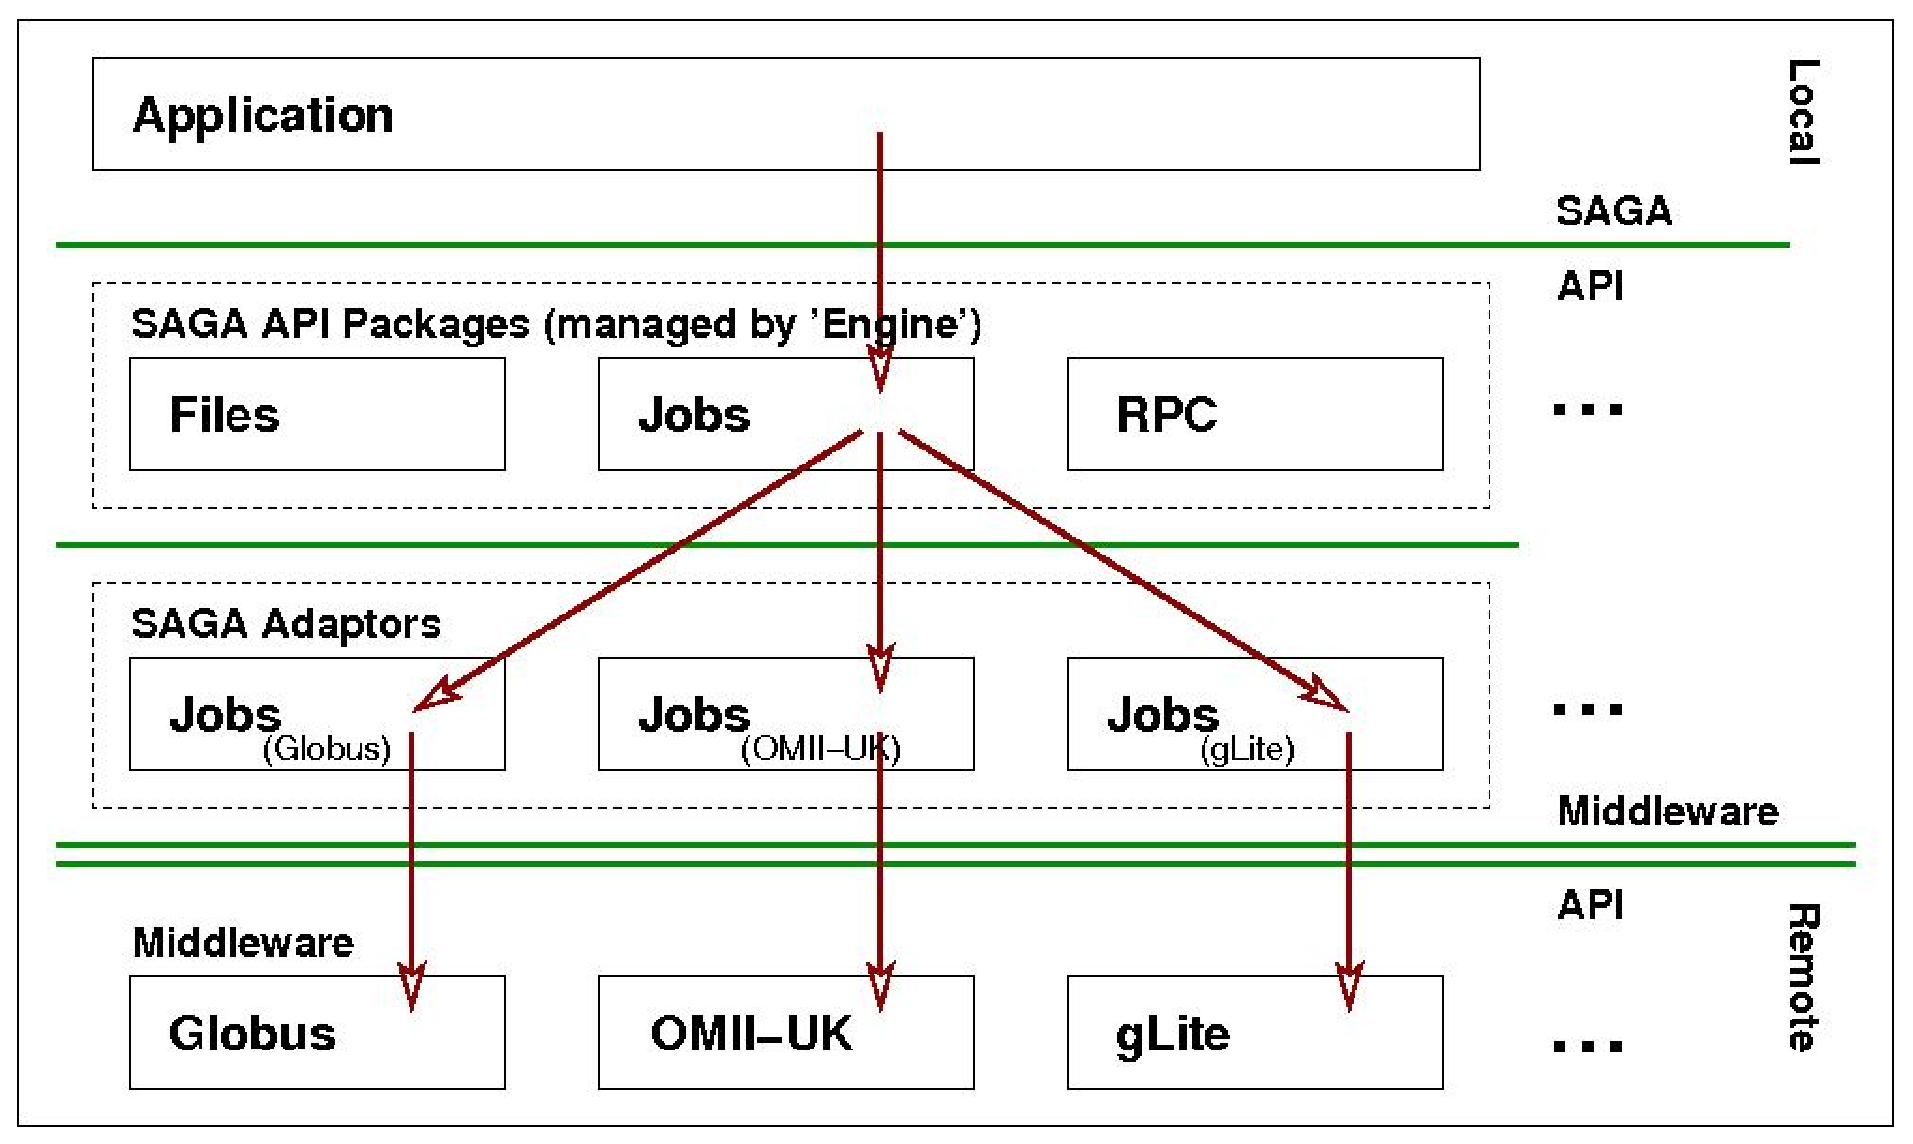
\includegraphics[width=0.47\textwidth]{images/saga_architecture}
  \caption{\label{fig:archi}
    Architecture: A lightweight engine dispatches SAGA 
    calls do dynamically loaded middleware adaptors.}
 \end{center}
\end{figure}

\subsection{Design Objectives}

	The Simple API for Grid Applications is, by definition, well ... \I{simple}. 
	This doesn't imply the implementation itself has to be simple. We made a major 
	effort to build	as much logic and functionality as possible into the 
	SAGA engine providing all the needed common functionality. This	enables the 
	user to extend it with minimal effort. On the other hand, 
	the library \I{is} designed to be easy to build, use, and deploy. 
	
	As described in the previous section, a SAGA implementation has to cope 
	with a multitude of different dynamic boundary conditions. A major design
	objective therefore was to maximize decoupling of different components
	of the developed library to allow for as much as possible \I{flexibility}, 
	\I{adaptability} and \I{modularity}.

	As the SAGA implementation is expected to be used on different platforms
	and operating systems we strive for maximal implementation \I{portability}. 

  The API should be \I{extensible} with minimal effort: ideally,
  adding a new API class is orthogonal to all other properties of the
  implementation, and immediately benefits from those.


\subsection{The Overall Architecture}

	To meet these goals we decided to decouple the library components
	in three dimensions. These three dimensions are completely orthogonal -- 
	the user of the library may use and combine these at free will and may 
	develop additional suitable components usable in tight integration with 
	the provided modules.

\subsubsection{Horizontal Extensibility -- API Packages}
\label{ssec:apipackages}

	The SAGA specification is object oriented and defines a set of API groups
	keeping objects of related functionality together (packages). Our implementation
	uses this functional grouping to define \I{API packages}.	The currently 
	defined packages are: file management, job management, remote procedure calls, 
  replica management, and data streaming. Each of 
	these packages constitutes a separate and independent module. 
	These modules depend only on the SAGA engine, the user is therefore free to 
	use and link only those modules actually needed by the application, minimizing 
	the memory footprint.
	
	New API packages are expected to be added in the future as the SAGA specification
	evolves. It is straightforward to add new packages since all common operations 
	needed inside these packages (as adaptor loading and selection, and method call routing) 
	are imported from the SAGA engine.  The creation of new packages is
  essentially reduced to:

  \begin{shortlist}
	   \item add the API (5) package files, and declare the classes,
	   \item reflect the SAGA object hierarchy (more details below, in
	   			 section~\ref{ssec:pimpl}), 
	   \item add class methods
  \end{shortlist}

  The declaration and definition of the API methods is greatly simplified by
  several macros, which essentially correspond directly to the methods
  SIDL specification.  We consider to (partly) automate the generation
  of new packages, by parsing the SIDL specification and generating the
  class stubs and class method specifications.  The user must then
  only add the required include files to get a full fledged,
  compilable and usable SAGA API implementation package. This approach will 
  allow us to generate other SAGA language bindings from the SIDL 
  specification as well, such as for the C and FORTRAN languages.
  
  Additionally we are using the Boost.Wave~\cite{wave_website} C++ preprocessor 
  and special \#pragma's implemented by this tool to pre-generate 
  partially macro expanded sources allowing to overcome the disadvantages 
	of plain macros, hence simplifying debugging and improving readability.
  
  % I have a perl script which does the essential part of that
  % generation process already - I stopped maintaining it as we
  % updated the packages, but will get it up to date at some point.  I
  % could actually create the old package types, only the inheritance
  % stuff and the impl initialization was missing :-) -- AM
	
\subsubsection{Vertical Extensibility -- Middleware Bindings}

	A layered architecture (see figure~\ref{fig:archi}) allows us to vertically decouple the SAGA 
	API from the used middleware. Separate adaptors, either loaded at 
	runtime, or pre-bound at link time, dispatch the different API
	function calls to the appropriate middleware. Most of the time
	there will be a separate set of adaptors for each type of middleware to 
	support. These adaptors implement a well defined capability provider
	interface (CPI) and expose that to the top layer of the library, which makes it
	possible to switch adaptors at runtime and hence to switch between 
	different (and even concurrent) middleware services providing the requested 
	functionality. The top library layer dispatches the API function calls 
	to the corresponding CPI function.
	
	The top library layer additionally contains the \I{SAGA engine} module,
  which implements:
	\begin{shortlist}
		\item core SAGA objects such as session, context, task or 
					task\_container -- these objects are responsible for the
          SAGA look\,\&\,feel, and are needed by all API packages;
		\item common functions needed to load and select matching 
					adaptors, to perform generic call routing from API 
					functions to the selected adaptor, to provide necessary
					fall back implementations for the synchronous and asynchronous
					variants of the API functions (if these are not supported by
          the selected adaptor).
	\end{shortlist}

	The dynamic nature of this layered architecture enables easy future 
	extensions by adding new adaptors, coping with emerging grid standards 
	and new or changed grid middleware.
	

\subsubsection{Extensibility for Optimization and Features} 

  Many features of the engine module are implemented by intercepting,
  analyzing, managing, and rerouting function calls between the API packages,
  where they get issued, and the adaptors, where they get executed
  and forwarded to the middleware.  To generalize that management
  layer, a PIMPL~\cite{pimpl} (Private Implementation) 
  idiom was chosen, and is rigorously
  used throughout the SAGA implementation.  That PIMPL layering allows
  for a number of additional properties to be transparently
  implemented, and experimen\-ted with, without any reflected change in
  either the API packages nor in the adaptor layers.  These features
  include:

	\begin{shortlist}
    \item generic call routing
	  \item task monitoring and optimization
    \item security management
    \item late binding
	  \item fallback on adaptor invocation errors
    \item latency hiding mechanisms
	\end{shortlist}

	The decoupling of these features from the API and 
  the adaptors succeeds, essentially, because these properties 
  affect only the IMPL side of the PIMPL layers.  

  Firstly, the private implementation classes all inherit from the same
  base class -- only that base class is handled in the central engine
  module, so the engine can automatically cope with new API packages
  and adaptors.  Secondly, all method calls are also handled
  generically in the engine.
  
  The engine module is hence fully generic, and loosely coupled to
  both the API and the adaptor layers.  Any changes to the engine, all
  optimization, latency hiding techniques, monitoring features etc.
  can be implemented in the engine generically, and are orthogonal to
  the API and adaptor extensions.  Hence, the extensibility of the
  engine represents the third orthogonal axis in the libraries
  extensibility scheme.

  % This is now described in 4.1.2 -- AM
  % 
	% Any of the package API functions are exposed in three variants: synchronous
	% asynchronous ans task based execution. The synchronous variant blocks
	% while the requested function is executed. On the other hand the asynchronous 
	% and task based variants immediately return a task instance encapsulating
	% the requested function call, whereas the task returned from the asynchronous 
	% call has already been star\-ted. The task returned from the task based 
	% function call needs to be started explicitely by calling the task::run() 
	% member.



  \section{Implementation Challenges\\ and Details}
    \label{sec:details}
    % $Header: /projects/VU-SAGA/Papers/saga_engine_2006/details.tex,v 1.17 2006/10/11 02:55:39 gallen Exp $

The following section will describe certain implementation details
of the SAGA C++ reference implementation. As will be described, the 
implementation gains its flexibility mainly from the combined
application of C++'s compile time and runtime polymorphism features,
i.e.\ template's and virtual functions respective.

\subsection{General Considerations}

  To achieve  maximum portability, platform independence and code
  reuse, the SAGA C++ reference implementation relies strictly on the
  Standard C++ language features, and uses the C++ Standard and Boost
  libraries where possible. 
  
\subsubsection{The SAGA task model}
\label{ssec:tasks}

  A central concept of the SAGA API design is the SAGA task
  model~\cite{saga-paper}, prescribing
  the form of
  synchronous and asynchronous method calls.  Essentially, each method
  call comes in three variants: as a \I{synchronous call} (executed 
  immediately), as a \I{asynchronous call}, and as a \I{task call}.  
  The latter versions of the calls return a \T{saga::task} class instance.  A
  \T{saga::task} thus represents an asynchronously running operation,
  and has an associated state (\T{New, Run\-ning, Finished, Failed}).  Task versions
  of the method calls return a \T{New} task, asynchronous versions
  return a \T{Run\-ning} task. %, i.e. the \T{run()} method was called on
  %that task.  
  For symmetry reason, we added a fourth, synchronous version of method
  calls, returning a \T{Finished} task.
  % i.e. \T{run()} and \T{wait()} have been called.
  The realization of the |saga::impl::task| class bases on a
  implementation of the \I{futures} paradigm, a concurrency abstraction 
  first proposed for MultiLisp~\cite{futures}.  
  The C++ rendering of the SAGA task model is shown in
  figure~\ref{src:tasks}.

\begin{figure}[!ht]
 \begin{center}
  \begin{mycode}[label=SAGA task model]
    string dest = "any://host.net//data/dest.dat";
    file   file  ("any://host.net//data/src.dat");

    // normal sync version of the copy method
    file.copy (dest);

    // the three task versions of the same method
    task t1 = file.copy <task::Sync>  (dest);
    task t2 = file.copy <task::ASync> (dest);
    task t3 = file.copy <task::Task>  (dest);

    // task states of the returned saga::task
    // t1 is in 'Finished' or 'Failed' state
    // t2 is in 'Running'              state
    // t3 is in 'New'                  state

    t3.run  ();
    t2.wait ();
    t3.wait ();
    // all tasks are 'Finished' or 'Failed' now
  \end{mycode}
  \up
  \up
  \caption{\label{src:tasks}
    The SAGA task model rendered in C++}
 \end{center}
\end{figure}

While we tried to absolutely minimize the use of template's in the 
API layer, it was decided to implement the different flavors of the API 
functions using function templates (see figure~\ref{src:tasks}). 
This makes the whole SAGA C++ implementation \I{generic} with respect to 
the synchronicity model, being another reason for providing 
two types of the synchronous function flavors: a direct and a task 
based one.

\subsubsection{The Object Instance Structure}
\label{ssec:pimpl}

As already mentioned, the SAGA API objects are implemented using the PIMPL idiom.
Their only essential member is a \T{boost::smart\_ptr<>} to the 
base class of the implementation object instance\footnote{\small We refer to the 
implementation side of the PIMPL layer as \I{impl classes} in this document}, 
keeping it alive. This makes them very 
lightweight and copyable without major overhead, and therefore storable in any 
type of container.

\begin{figure}[!ht]
 \begin{center}
  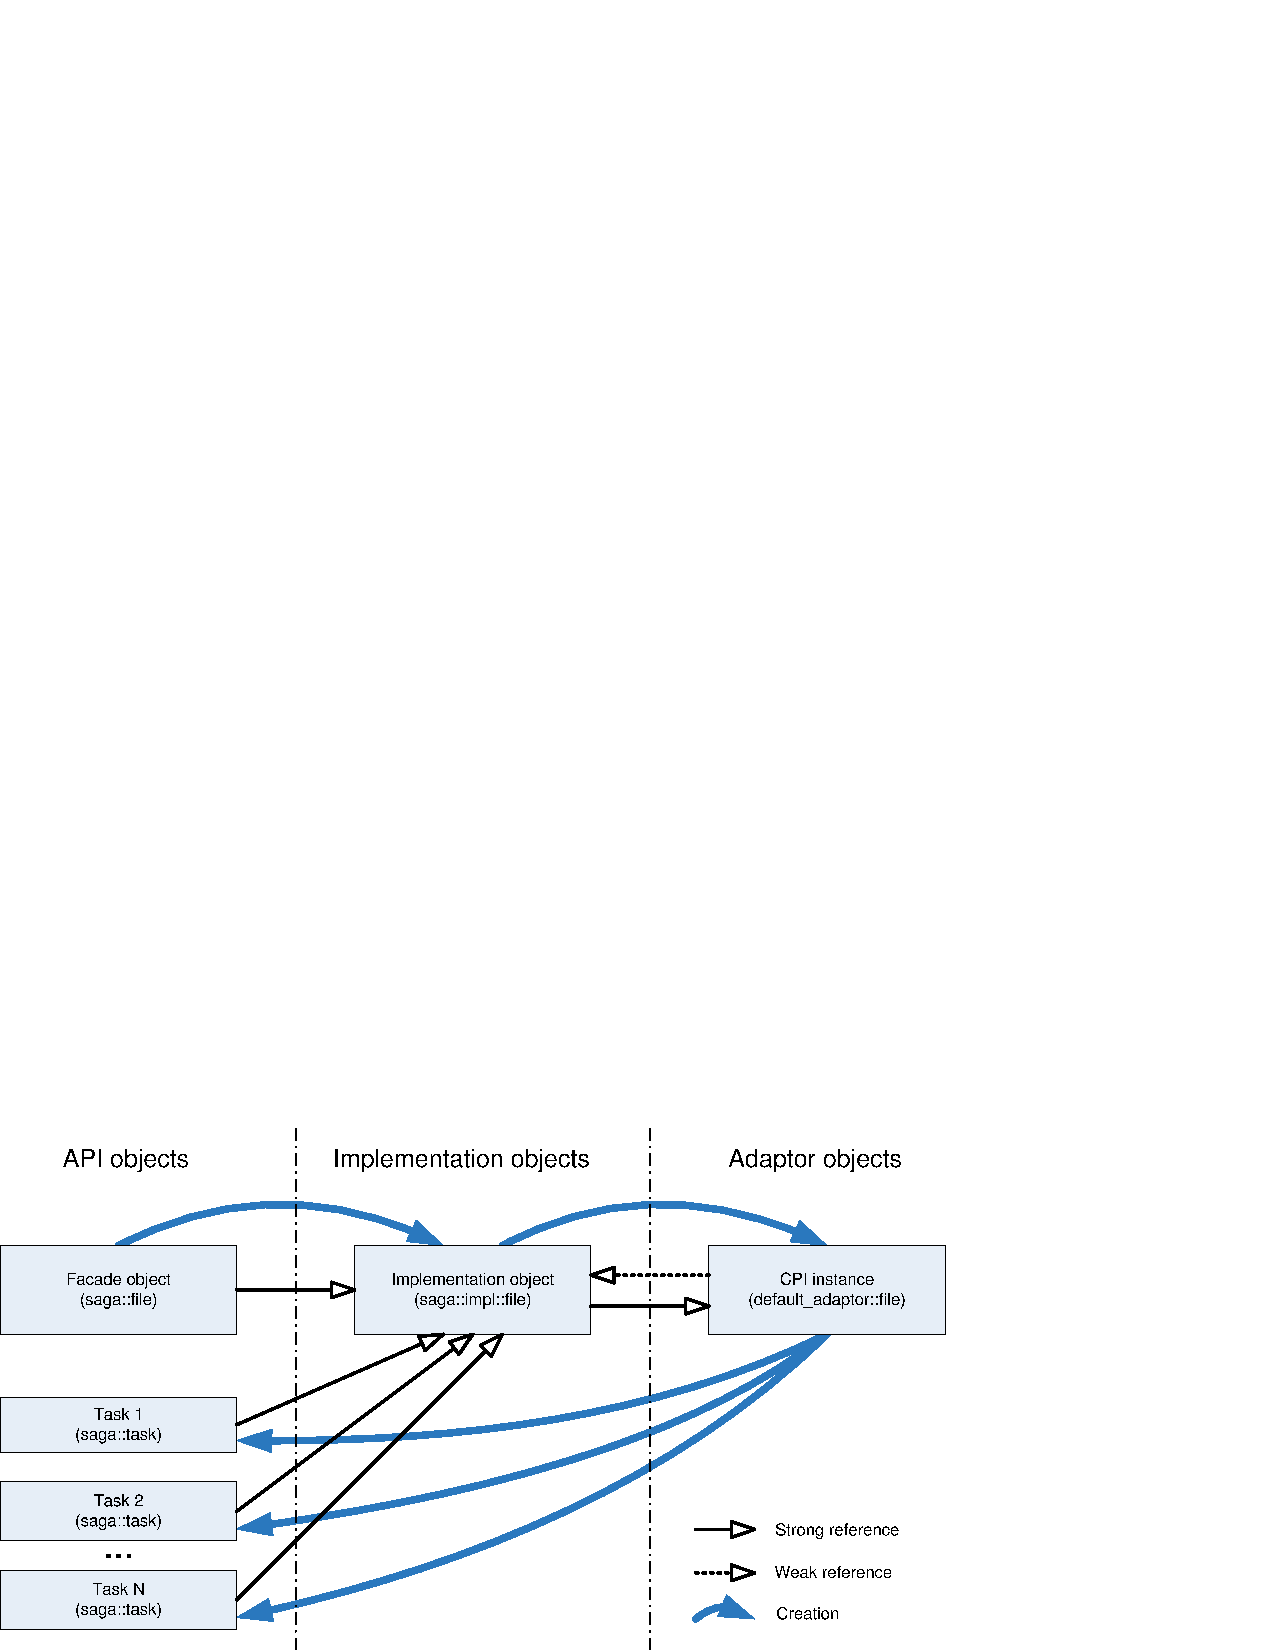
\includegraphics[width=0.47\textwidth]{images/object_structure}
  \up
  \caption{\label{fig:object_structure}
    Object instance structure: Copying a API object instance means sharing 
    state, returned tasks keep implementation alive.}
 \end{center}
\end{figure}

As shown in figure~\ref{fig:object_structure}, any API object instance creates
the corresponding impl instance holding all the instance data
of the SAGA object instance 
Copying of an API instance therefore shares this state between the copied 
instances.
This behavior is consistent with anticipated handle based SAGA language bindings 
(e.g. in C or FORTRAN), where copying the handle representing a SAGA 
object instance naturally means sharing the internal instance data as 
well\footnote{\small A polymorphic \T{saga::object::clone()} method is, however, part 
of the SAGA API, and allows for explicit deep copies of API objects, 
forcing the instance data to be copied as well.}.  

Due to the shared
referencing after copies, the impl instances can be kept alive by objects
which depend on their state -- for example, a task keeps the objects
alive for which they represent a asynchronous method call (see
figure~\ref{fig:object_structure}).

The call sequence for creating a SAGA API object instance is shown in
figure~\ref{fig:object_creation}.  Whenever needed, the implementation
creates a CPI object instance implemented in one of the adaptors.
The process of adaptor selection and CPI instantiation is injected into the 
API packages by the macros mentioned before (see section~\ref{ssec:apipackages}).

\begin{figure}[!ht]
 \begin{center}
  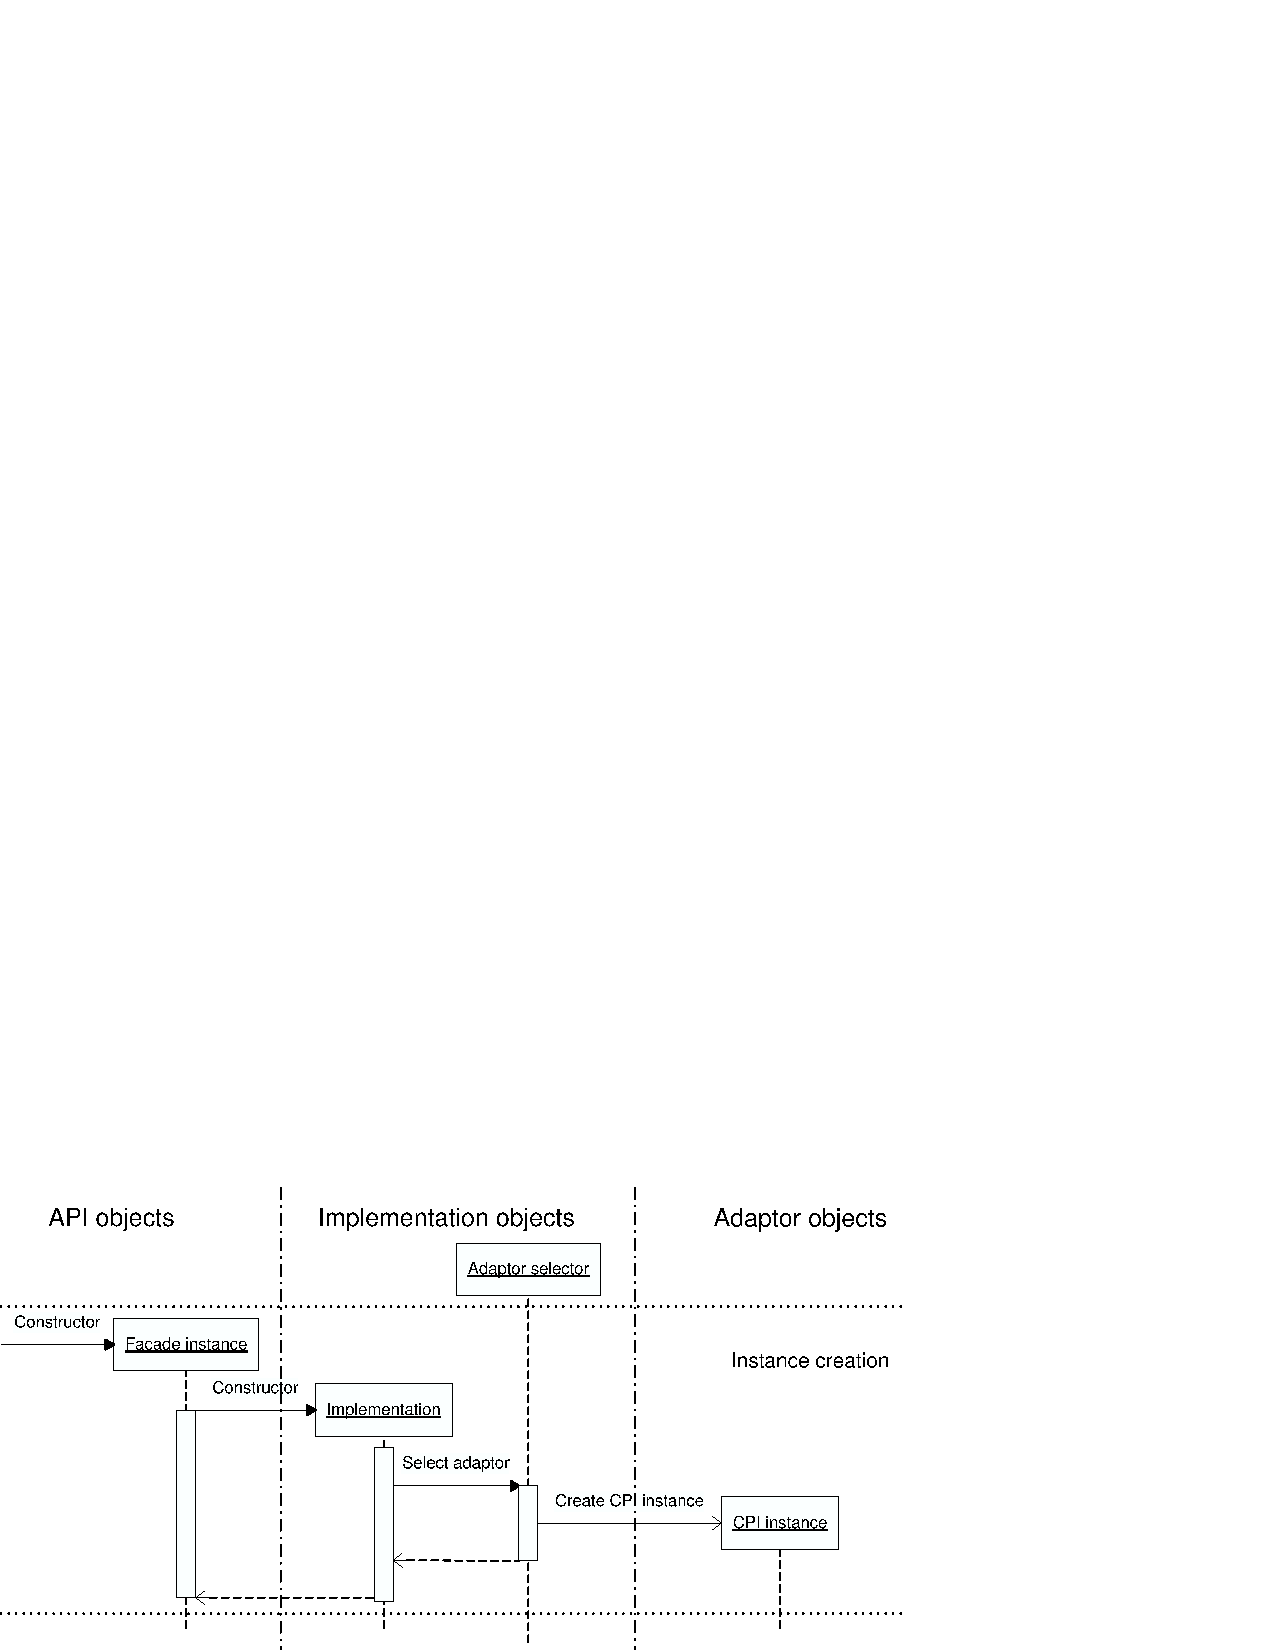
\includegraphics[width=0.47\textwidth]{images/object_lifetime_creation}
  \up
  \caption{\label{fig:object_creation}
    Object creation: Sequence diagram depicting the creation of all
    components as showed in figure~\ref{fig:object_structure}. Note, how
    the call is intercepted by a SAGA engine module component to select 
    a appropriate adaptor.}
 \end{center}
\end{figure}

\up
\up
\subsection{Inheritance and PIMPL}

An interesting problem in the strict application of the PIMPL
mechanism lies in the API object hierarchy:  the \T{saga::file} class
for example inherits the \T{saga::ns\_entry} class, which inherits the
\T{saga::object} class.  Additionally, the SAGA specification requires
all these classes to implement additional interfaces.  Now, the PIMPL
paradigm requires all class instances to own exactly \I{one} impl
pointer\footnote{\small{In fact the impl pointer stored in any \T{saga::object}
instance is a \T{boost::smart\_ptr<saga::impl::object>}, i.e. a reference
to the very base class of the implementation object hierarchy.}}, and are 
built using single inheritance only, otherwise we would face object slicing 
problems when copying around the base classes only. The solution is (1) to
add the required interfaces to the most derived classes by duplication
the interface functions, and (2) to up-cast the impl reference stored in the
base class whenever needed.

\begin{figure}[!ht]
 \begin{center}
  \begin{mycode}[label=Constructors in the saga::file hierarchy]
  // saga::file constructor
  file::file ([args])
  :  ns_entry (new saga::impl::file ([args]))  {}
  
  // saga::ns_entry constructor
  ns_entry::ns_entry (saga::impl::ns_entry* impl)
  :  saga::object (impl) {}
  
  // saga::object constructor
  //  'impl_' is a boost::smart_ptr<saga::impl::object>
  object::object (saga::impl::object* impl)
  :  impl_ (impl) {}
  \end{mycode}
  \up
  \up
  \caption{\label{src:implcon}
    Realizing inheritance in PIMPL classes (simplified).  Only the
    \T{saga::object} base class owns an impl pointer.}
 \end{center}
\end{figure}

API classes access the impl pointer through \T{get\_impl()}, which, in
derived classes, implies a static up-cast for the base class' impl
pointer.  

The implementation objects resemble the API object hierarchy.  These
are also derived from a common base class and contain, somewhere in
their own hierarchy, similar objects to the API objects.  The
\T{saga::impl::file} class\footnote{\small{The \T{saga::impl::file}
class for example is the implementation equivalent to the
\T{saga::file} class, as we kept all API classes in \T{namespace~saga}
and all corresponding implementation classes in
\T{namespace~saga::impl}.}} inherits the \T{saga::impl::ns\_entry}
class, which inherits the implementation specific
\T{saga::impl::proxy} class, which is derived from the common
\T{saga::impl::object} class.  Thus, the class hierarchy on the
implementation side of the PIMPL paradigm reflects the API side of the
class hierarchy, ensuring the correct casting behavior in the
\T{get\_impl()} methods.


\subsection{State Management}

Section~\ref{ssec:pimpl} discussed object state, in relation to
state sharing of objects after shallow copies.  Here we describe the object
state management of the SAGA implementation in more detail, since state
management is a central element on several layers.
On a different layer, the adaptors represent
operations on the object instances, and need to maintain state as well.
At the adaptor level this is complicated by the fact that the object state can (and in
general will) be changed by several adaptors (remember: adaptors are selected
at runtime, and may change for each API function invocation).  For state 
management, we hence distinguish between three types of state information.

\begin{shortlist}
	\item \I{Instance data} represent the state of API objects (e.g. file name, 
			file pointer etc.). These are predefined and not amendable by the adaptor
			as they represent common data either passed from the constructor,
			or needed for consistent state management on the API level.
	\item \I{Adaptor data} represent the state of CPI objects (e.g. open connections)
      and are shared between all instances of all CPI object types
			implemented by 
			a single adaptor and corresponding to a single adaptor instance. 
	\item \I{Adaptor-instance data} represent the state shared between all CPI 
			instances created for a single API object and implemented by the same 
			adaptor (e.g. remote handles). 
\end{shortlist}

The lifetime of any type of the state information is maintained by the SAGA engine 
module, which significantly simplifies the writing of adaptors.

All three types of state information are carefully protected from race 
conditions potentially caused by the multithreaded nature of the implementation.
We provide helper classes simplifying the 
correct locking of the instance data. 
This uniform state management enables 
object state persistency in the future, with minimal impact on the 
code base.

\subsection{Generic Call Routing}
\label{ssec:routing}

The essential idea of the implemented generic API call
routing mechanism is to represent the calls as abstract objects, and
to redirect their execution depending on several attributes 
and the adaptor suitability.  For example,
an asynchronous method call for a |saga::file| instance is preferably
directed to a asynchronous file adaptor, or, if such is not available,
to a synchronous file adaptor, wrapping it in a thread,
or, returns an error otherwise (|NotImplemented|).

This routing mechanism allows for (1) trivial (synchronous) adaptor 
implementations, (2) late binding (differents adaptor can be selected
for each call, even on the same API object instance), (3) variable adaptor 
selection strategies (based on adaptor meta data, user preferences, 
and heuristics), and (4) latency hiding (bulk optimization~\cite{CS_Hirmer_06a}, 
or automatic load distribution over multiple adaptors). 
Figure~\ref{fig:object_functioncall} is depicting the injection of the
call routing mechanism by the SAGA engine.

\begin{figure}[!ht]
 \begin{center}
  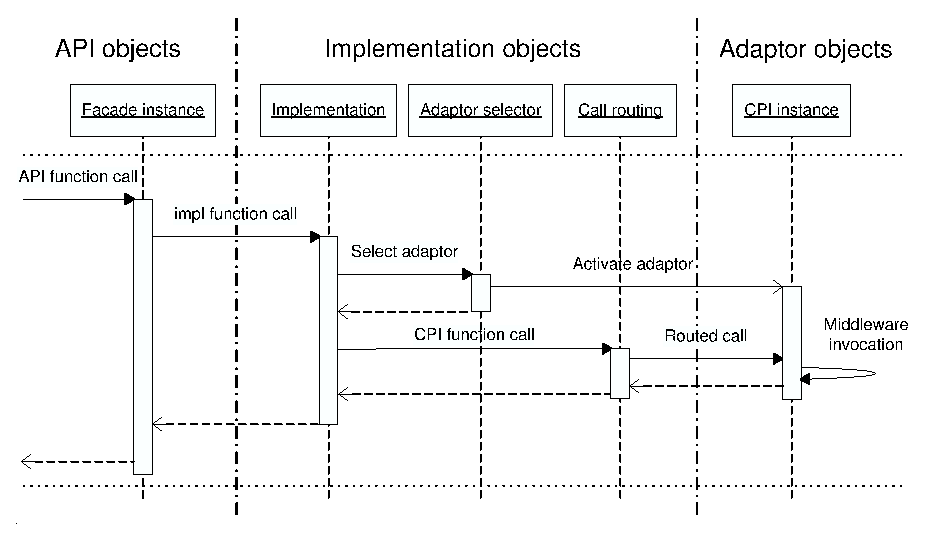
\includegraphics[width=0.47\textwidth]{images/object_lifetime_functioncall}
  \up
  \caption{\label{fig:object_functioncall}
    API function call: Diagram illustrating the execution sequence through 
    the different object instances during a call to any adaptor supplied 
    function.}
 \end{center}
\end{figure}

\up
All SAGA API methods come in synchronous and asynchronous flavors
(see section~\ref{ssec:tasks}).
To avoid, that adaptors need to implement
both flavors, we provide fallback implementations in the
SAGA engine.
The synchronous behavior is modelled by 
executing the the asynchronous implementation and waiting
for it to finish.  The asynchronous wraps the synchronous
implementation into a thread representing the asynchronous 
remote operation.

Even if this approach has a couple of drawbacks (it is not really asynchronous,
the middleware call still blocks, causing lock problems if implemented badly, and
tasks are not able to survive the application life time), the mechanism 
simplifies adaptor implementations
greatly, as most of the existing grid middleware is \I{not}
fully asynchronous anyway.

\subsection{Adaptor Selection}

The selection of suitable adaptors at runtime  is a central
component in the implementation (see
figure~\ref{fig:object_functioncall}).  It is, a very simple
mechanism: on loading, the adaptor components register their
\I{capabilities} in the adaptor registry.  If a method is to be
executed, the adaptor selector searches that registry for all 
suitable adaptors, orders them, and tries them one-by-one,
until the method invocation succeeds. The adaptor selection is 
routed through SAGA engine, generically implementing this for 
any API function.

To overcome the limitations of this approach (several CPI instances 
have to be created, remote operations add  additional latencies), our 
library allows adaptors to specify additional, key/value
based meta data, and also allows to exchange the adaptor selection
component.

\subsection{Utilization of Macros}
\label{ssec:macros}

Our SAGA implementation makes extensive use of C++ preprocessor
macros.  This might be perceived as a design flaw, at least by
some readers, and we were very hesitant to utilize macros
extensively.  However, the benefits for the end user
and other programmers(!) seem currently to outweigh the problems, 
such as limited debugging abilities.
mentioned in section~\ref{ssec:apipackages}, We are using Boost.Wave~\cite{boost_website}
features to pre-generate partially macro expanded sources to overcome 
the disadvantages of plain macros, hence simplifying debugging and 
improving readability.


  \section{Lessons Learnt --\\ Implementation Properties}
    \label{sec:props}
    % $Header: /projects/VU-SAGA/Papers/saga_engine_2006/properties.tex,v 1.4 2006/08/13 18:01:00 hkaiser Exp $

The paper so far motivated the design objectives of the SAGA C++
Reference implementation, and described several implementation
techniques used to meet these design objectives.  This section will
summarize the resulting properties of the SAGA implementation from an
end user perspective, and will motivate further developments and
extensions.


\subsection{Uniformity over Programming Languages}
\label{ssec:lang}

 The SAGA API specification is language independent -- however, it is
 a declared goal to define language bindings which both, if possible,
 provide a language-native look\,\&\,feel to the user of the API, and
 strive for syntactic and semantic similarity over all SAGA language
 bindings.  One of the consequences of that goal is that the API
 specification does not use templates, as that was thought too
 difficult to express uniformly over many languages.  Also, the
 specification tries to be concise about object state management, and
 hence also expresses semantics for shallow and deep copies.

 Our implementation follows the specification closely, naturally.  Furthermore,
 it is designed to accommodate wrappers in other languages, so as to
 provide the same semantics, and similar look\,\&\,feel to other
 language bindings.  In fact, a Python wrapper for our library is in
 alpha stadium, and we consider similar thin wrappers to provide
 bindings to C, Fortran, Perl, and possibly others.

 From a different point of view, we find it extremely convenient to be
 able to implement \I{adaptors} in different languages as well.  The
 Grid Application Toolkit (GAT, \cite{gat}), a C-based API predecessor
 of SAGA,  already allows adaptors in different languages, and we
 consider to implement similar mechanisms to allow Python or C based
 adaptors for our implementation as well.  In particular Python based
 adaptors have shown to be extremely useful for rapid prototyping of
 middleware bindings for GAT.

\newpage
\subsection{Genericity in respect to Middleware, and
            Adaptability to Dynamic Environments}

 The dynamicity of grid middleware was mentioned a number of times
 already, as it \I{is} a very central and dominating property of grid
 environments.  The described adaptor mechanism used in our
 implementation to bind to diverse middleware binding addresses that
 point.  Additionally, late binding, fall back mechanisms, and
 flexible adaptor selection allows for additional resilience against
 an dynamic and evolving run time environment.  It must be noted,
 however, that adaptors need to deploy mechanism like resource
 discovery, and need to implement fully asynchronous operations, if
 the complete software stack is to be able to cope with dynamic grids
 -- our SAGA implementation usability will be severely impacted if the
 quality of adaptors undermines the libraries mechanisms.


\subsection{Modularity makes the Implementation \\Extensible}

 Section~\ref{ssec:macros} has shown in some detail that our SAGA
 implementation is well able to cope with the expected evolution and
 extension of the SAGA API.  On the other hand, the adaptor mechanism
 allows for easy extensions of the library, to provide additional
 middleware bindings.  In fact, the major future work for our SAGA
 implementation will be to provide multiple sets of stable adaptors
 for the major grid environments.  We expect, however, that that task
 requires massively more effort than the implementation of the
 presented library, and we very much hope for the support of grid
 middleware vendors to provide, and (above all) maintain these
 adaptors.  Ideally we would actually wish that middleware vendors
 \I{implement} adaptors to our SAGA implementation, and deliver them
 as part of their client side software stack.  If that scenario will
 ever come to pass remains to be seen -- it would certainly help to
 get the SAGA API a very wide user community.


\subsection{Portability and Scalability}

 Heterogeneous distributed systems naturally require por\-table code
 bases.  We think that our library implementation is in fact very
 portable, as we strictly adhere to the C++ standard and portable 
 libraries.  In fact,
 we currently develop the library on Windows and Linux concurrently,
 so we are confident that we are able to cover the two
 major target platforms without any problems -- but we don't expect
 (and currently don't encounter) any problems on other platforms.  It
 must be noted, however, that the portability of our SAGA implementation
 depends on the portability of the adaptors, and hence on the portability 
 of the grid middleware client interfaces, being the much greater problem 
 if compared to the library code itself.

 Distributed applications are quite often sensitive to sca\-lability
 issues, in particular in respect to remote communications.  As SAGA
 introduces a number of communication mechanisms, scalability concerns
 are naturally also raised in respect to SAGA implementations.
 Firstly it must be said, that the SAGA API is not targeting
 high performance communication schemes, but rather tries to stick to
 simple communication paradigms -- in no sense does SAGA intent to
 replace MPI or other distributed communication libraries.  Having
 said that, our design allows for zero-copy implementations of the
 SAGA communication APIs, and also allows for fast asynchronous
 notification on events -- both are deemed critical for implementing
 scalable distributed applications.  
 
 %Again, our library depends on
 %hi-quality adaptor implementations to utilize these features.


\subsection{Simplicity for the End User}

 SAGA is \I{designed} to be simple to use.  However,
 simplicity of use of an API is not only determined by its API
 specification, but also by its implementation: simple deployment 
 and configuration, resilience against lower level failures,
 adaptability to diverse environments, stability, correctness, and
 peaceful coexistence with programming paradigms, tools and libraries
 are some of the characteristics which need attention while
 implementing the SAGA API.  
 
 It is a challenging task to keep a library implementation as this one
 simple in itself, meaning to have readable code, with a limited
 amount of magic.  Again, a very modular approach helps here very
 much, in out opinion.  For example, it is very simple to hide the
 generic call routing, or the adaptor selection, in the engine module,
 as these features are not usually exposed to the user or adaptor
 programmer.  However, we think that modeling these central properties
 as modules increases the readability and maintainability of the code
 significantly.  

 The SAGA API implicitly introduces a concurrent programming model,
 due to its notion of asynchronous operations, or tasks.  The C++
 language binding of the API, and our implementation, allows to combine
 that model with arbitrary mechanisms for managing concurrent program
 elements (i.e. to ensure object state consistency in all
 circumstances, to ensure thread safety, and to allow for application
 level semaphores and mutexes).


% \subsection{Meeting the Design Objectives}
% 
% Our most important objective was to design a state-of-the-art grid application 
% framework satisfying the majority of user-needs while staying as flexible 
% as possible, both towards further API extensions (due to extensions of the SAGA API), 
% towards emerging grid middleware frameworks, services, and standards, as well as 
% towards its usability in different usage scenarios as synchronous, asynchronous,
% task based etc.
% 
% %Simplicity: easy to use, install, administer and maintain 
% \subsubsection{Simplicity for the End User}
% A major design goal of our implementation was \emph{simplicity} -- not
% for the implementation itself, but for the users of this
% implementation. In particular, this SAGA implementation should,
% be easy to install, use, administer and maintain, especially and even by 
% non-computer scientists. In our experience, this kind of simplicity is 
% a major precondition for a broad acceptance amongst grid users. 
% 
% The interfaces exposed towards the user of our library are defined by the
% SAGA strawman API~\cite{saga_spec} and hence by definition very simple, compared
% to complicated grid middleware interfaces, hidden by our implementation.
% 
% The SAGA C++ reference implementation potentially provides access to every
% possible grid middleware, by abstracting from middleware specific details.
% Only relevant details are defined in the SAGA API specification and our implementation 
% links the abstract and middleware independent specification to lower level
% middleware frameworks. Our implementation meets this requirement by extensively using
% the adaptor pattern~\F{cite Gamma et al.}. Middleware frameworks make their functionality
% available through adaptor libraries used by the SAGA C++ core on the fly
% by using a plug in mechanism.
% 
% During compile time it is normally not known which grid middleware frameworks will be 
% available at runtime. Furthermore, because of the highly dynamic nature of 
% distributed systems we cannot rely on the existence of required middleware services. 
% The only way to deal with this kind of dynamics is to implement trial and error 
% mechanisms ensuring a maximum of coverage of potential functionality: i.e. the only way 
% to ensure a certain middleware service is available is to try a required operation and
% verify it actually succeeded.
% 
% A dynamic middleware recognition and selection was required. Our implementation
% analyses available grid middleware frameworks and their adaptors and loads them dynamically
% at the moment of function execution. The most suitable
% adaptor is chosen to execute a given operation. As grid environments are dynamically
% changing, execution failures may occur frequently. If a given grid middleware fails to
% execute a given operation, the next most suitable adaptor is selected and executes the
% operation of interest. 
% 
% This whole mechanism is absolutely transparent for the library user, only the failure
% of all available frameworks to execute a given operation is reported to the invoking
% application.
% 
% The same dynamic plug-in mechanism provides also the means for simplicity in terms
% of maintenance and administration. As new middleware framework can be added dynamically
% -- even during runtime of an application -- no recompilation is required. The same holds
% for SAGA scope extensions. In both cases additional shared libraries are copied into
% the current installation and recognized and used by the SAGA core on the fly.
% 
% 
% % should this go into this paper? Is more a SAGA feature, than a feature of this impl? --STH
% %\subsubsection{Uniformity over Programming Languages}
% %As every scientist should potentially be able to use our
% %implementation, the target user group originates from a large variety
% %of research domains, each with their own programming habits and
% %language preferences. Hence it is highly desirable to provide the
% %widest possible range of \emph{uniformly} supported programming
% %language bindings. So far, our implementation provides bindings for
% %C++ and Python.  Language bindings for FORTRAN, Perl and others are
% %planned.  A separate Java reference implementation is currently
% %developed by the Open Middleware Infrastructure Institute (OMII-UK).
% 
% 
% %Uniformity: provides support for different application programming languages 
% \subsubsection{Uniformity over Programming Languages}
% \F{Explain constraints resulting from this SAGA requirement: no templates in the API,
% shallow copy semantics of API objects, ...anything else? -- HK}
% 
% %Genericity: adds support for different grid middleware, even
% %concurrent ones
% \subsubsection{Genericity in respect to grid Middleware}
% As different user groups use different grid middleware frameworks, another objective was 
% to enable the usage of these different middleware frameworks of choice through the means 
% of SAGA, while benefiting from its simplified and easy to use API in a \emph{generic}
% way.  Our implementation allows to use multiple grid middleware frameworks in parallel, 
% and even to chose the most appropriate one on the fly, to execute any required operation.
% 
% As already outlined in the above paragraph, our implementation is able to deal with
% every kind of middleware, if an appropriate adaptor (as shared library) exists, which
% is then used dynamically.
% 
% The adaptor loading and selection is of generic nature, both in terms of high-level
% functionality (file transfer as well as job submission etc.) as well as in terms of
% middleware support. This leads hence to a mapping of $n$ sets of API functionality
% to $m$ different middleware frameworks.
% 
% %Transparency: contains mechanisms for the same application (source)
% %code to run on a variety of systems ranging from laptops to HPC
% %resources Adaptability: orientation towards dynamic and adaptive
% %grid-aware applications Modularity: provides a framework easily
% %extendable 
% %\newpage
% 
% %Adaptability: orientation towards dynamic and adaptive grid-aware applications 
% \subsubsection{Adaptability to Dynamic Environments}
% 
% grid computing is defined as distributed computing with a focus on
% highly dynamic environments~\cite{CS_Foster01a}: any application running in grids
% must be aware of the volatile and dynamic nature of the environment.  Our
% implementation hides that behavior from the application layer as far as
% possible, and provides dynamically loadable extensions to cope with the changing
% middleware representation. That plug in mechanism is present on different layers
% of the implementations architecture:  new API packages can be added at compile
% time, new middleware bindings can be added at runtime, and the implementation
% can switch these middleware bindings between any two calls, for flexibility and
% fail safety.
% 
% %Modularity: provides a framework easily extendable 
% \subsubsection{Modularity makes the implementation Extensible}
% These plug in mechanisms have well defined interfaces, which allow middleware
% vendors and research projects to easily extend the reference implementation in 
% a \emph{modular} way, with both domain specific API packages, and with additional 
% middleware bindings.
% 
% \subsubsection{Portability and Scalability}
% The overall implementation is highly \emph{portable and platform independent}.  All
% operations are inherently asynchronous, even if this is not supported by the
% underlying middleware.  Bulk operations are automatically optimized, but need
% middleware support. The overall overhead introduced by the library is
% neglect able to any overhead introduced by the inherent latencies of grid
% environments.
% 
% In order to keep the implementation as portable and platform independent as possible, 
% we mainly rely on the strict usage of Standard C++ language features only, the usage 
% of Boost libraries wherever possible as well as the C++ Standard Library.
% 
% 
% 


	\section{Future Work}
		\label{sec:futurework}
		
	 As repeatedly said, the work on appropriate middleware adaptors will
	 undoubtedly require significant resources in the future -- but
	 without those, the SAGA API will not be usable in real grid
	 environments.  We will work on simplifying adaptor creation,
	 integration and maintenance, and hope for support from the OpenSource
	 community, and from grid middleware vendors.  We deem adaptor
	 development and support more important than the API development
	 itself.
	
	 In parallel, we will strive to provide other language bindings to our
	 implementation, as motivated in section~\ref{ssec:lang}, and want also
	 allow adaptors in various programming languages.  Finally, we plan to
	 apply further generic latency hiding techniques, and to experiment
	 with other API implementations in our framework.

  \section{Conclusion}
    \label{sec:Conclusion}
    % $Header: /projects/VU-SAGA/Papers/saga_engine_2006/conclusion.tex,v 1.10 2006/10/11 02:55:39 gallen Exp $

We have described the C++ reference implementation of the SAGA API,
which is designed as a generic and extensible API framework:  it
allows for the extension of the SAGA API,
easily usable for other APIs); 
it allows for run-time extension of
middleware bindings, 
and it allows for orthogonal optimizations and features,
such as late binding, diverse adaptor selection strategies, and latency
hiding.  The used techniques enable
these features, amongst them the application of the PIMPL paradigm for
a complete class hierarchy and generic call routing.

These implementation techniques incur a certain overhead, however, in
grid environments the runtime overhead is usually vastly dominated by
communication latencies, so that \I{\B{this} overhead does not
matter}.  The lesson learned is that distributed environments
\I{allow} for fancy mechanisms, which are too expensive in local
environments.  Fail safety and latency hiding mechanisms are
more important than, for example, virtual functions, late
binding, and additional abstraction layers.  


% -------------------------------------------------------------------

  \section{Acknowledgments}
  \label{sec:ack}
  
  We thank Thorsten Sch\"utt for his work on Futures; Michel Zsandstra
  and Vladimir Prus for their initial work on dynamic loading; the SAGA 
  groups in OGF for their work on the SAGA specification; the
  Lousisiana State University, the Vrije Universiteit Amsterdam, and
  the XtreemOS project for funding our work.
  % I have to mention XtreemOS from now on...

% -------------------------------------------------------------------

\bibliographystyle{unsrt}
\bibliography{saga_engine}

\end{document}

